%%%%%%%%%%%%%%%%%%%%%%%%%%EJERCICIO 8b %%%%%%%%%%%%%%%%%%%%%%%%%%%
\textbf{Solución b.}\\
	%La tabla irá centrada
	\begin{center}
		\renewcommand{\arraystretch}{1.5}% Márgenes de las celdas
		% Creación de la cuadrícula de 2 columnas
		\begin{longtable}[H]{|c|c|}
			% Creamos una línea horizontal
			\hline
			% Definimos el color de la primera fila
			\rowcolor[HTML]{FFB183} 
			\hline
			%%%%% INICIO ASIGNACIÓN FECHA FOCAL %%%%%%%
			%%%%%%%%%% INICIO TÍTULO
			% Lo que se hace aquí es mezclar las 2 columnas en una sola
			\multicolumn{2}{|c|}{\cellcolor[HTML]{FFB183}\textbf{1. Asignación período focal}} \\ \hline
			%%%%%%%%%% FIN TÍTULO
			%%%%% INICIO DECLARACIÓN DE VARIABLES %%%%%%%
			\multicolumn{2}{|c|}{$pf : 0 \; \textit{psv}$} \\ \hline
			\hline
			%%%%%%%%%% INICIO TÍTULO
			% Lo que se hace aquí es mezclar las 2 columnas en una sola
			\multicolumn{2}{|c|}{\cellcolor[HTML]{FFB183}\textbf{2. Declaración de variables}} \\ \hline
			\hline 
			%%%%%%%%%% FIN TÍTULO
			%%%%%%%%%% INICIO DE MATEMÁTICAS
			% Cada & hace referencia al paso de la siguiente columna
			\cellcolor[HTML]{FFB183}\textbf{Valores monetarios} & 
			\cellcolor[HTML]{FFB183}\textbf{Valores no monetarios} \\ \hline
			$L = 60{.}000 \; \text{COP}$ & $m = 2 \; \textit{psv}$ \\ 
			$H = 25{.}000 \; \text{COP}$ & $n = 6 \; \textit{psv}$ \\ 
			$ $ & $i = 16\% \; \textit{psv}$ \\ \hline

			%%%%%%%%%% FIN DE MATEMÁTICAS
			%%%%% FIN DECLARACIÓN DE VARIABLES

			\rowcolor[HTML]{FFB183}
			\multicolumn{2}{|c|}{\cellcolor[HTML]{FFB183}\textbf{3. Diagrama de flujo de caja}} \\ \hline
			\multicolumn{2}{|c|}{ 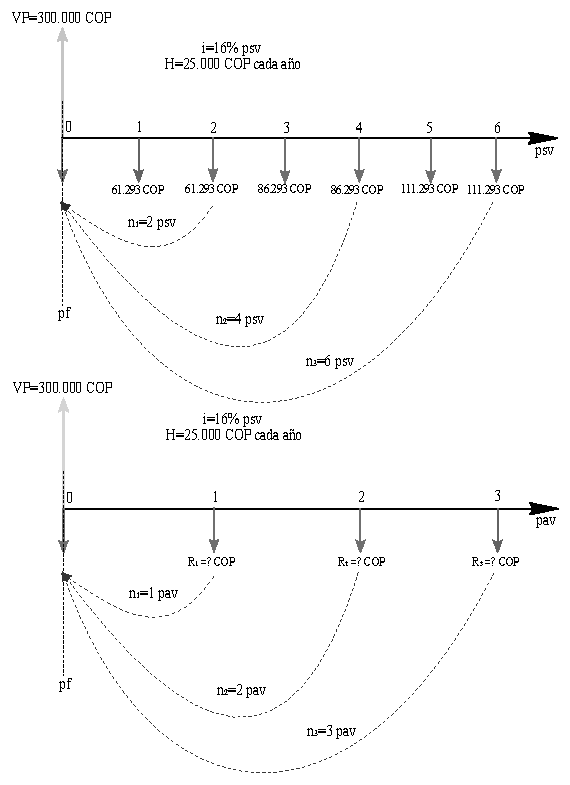
\includegraphics[trim=-78 -5 -78 -5]{7_Capitulo/img/ejemplos/8/8_2.pdf} } \\ \hline
			%%%%% INICIO FLUJO DE CAJA
			\rowcolor[HTML]{FFB183}
			\multicolumn{2}{|c|}{\cellcolor[HTML]{FFB183}\textbf{4. Declaración de fórmulas}} \\ \hline
			%%%%%%%%%%%%% FIN INSERCIÓN DE IMAGEN
			%%%%% FIN FLUJO DE CAJA

			\multicolumn{2}{|c|}{ $VP = R \frac{1-(1+i)^{-n}}{i} $ Valor presente de serie uniforme vencida } \\ 
			\multicolumn{2}{|c|}{ $VF = \frac{(1+i)^{-n}-1}{i} $ Valor futuro de serie uniforme vencida } \\ \hline
			
			%%%%%% INICIO DESARROLLO MATEMÁTICO
			\rowcolor[HTML]{FFB183}
			%%%%%%%%%% INICIO TÍTULO
			\multicolumn{2}{|c|}{\cellcolor[HTML]{FFB183}\textbf{5. Desarrollo matemático}} \\ \hline
			%%%%%%%%%% FIN TÍTULO
			%%%%%%%%%% INICIO MATEMÁTICAS
			\multicolumn{2}{|c|}{ $ L = \frac{ 25{.}000 \; \text{COP} (1 + 0{.}16)^{2} - 1}{0{.}16} = 54{.}000 \; \text{COP}$ } \\ 
			\multicolumn{2}{|c|}{ $ r_{1} = r_{2} = 61{.}293{,}00 \; \text{COP} $ } \\ \hline

			%%%%%%%%%% FIN MATEMÁTICAS
			%%%%%% FIN DESARROLLO MATEMÁTICO
			%%%%%% INICIO RESPUESTA
			\rowcolor[HTML]{FFB183}
			%%%%%%%%%% INICIO TÍTULO
			\multicolumn{2}{|c|}{\cellcolor[HTML]{FFB183}\textbf{6. Respuesta}} \\ \hline
			%%%%%%%%%% FIN TÍTULO
			%%%%%%%%%% INICIO RESPUESTA MATEMÁTICA
			\multicolumn{2}{|c|}{ 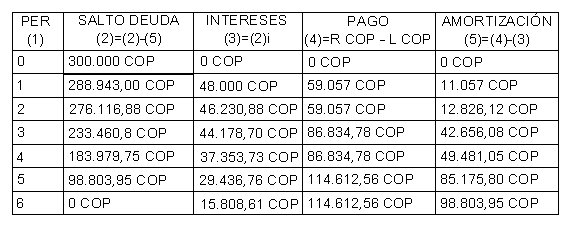
\includegraphics[trim=-78 -5 -78 -5]{7_Capitulo/img/ejemplos/8/8_2_2.pdf} } \\ \hline
		\end{longtable}
	\end{center}
%%%%%%%%%%%%%%%%%%%%%%%%%%FIN EJERCICIO 8b %%%%%%%%%%%%%%%%%%%%%%%%%%%
